\documentclass[10pt, letterpaper]{report}
% !TeX program = xelatex
%==================PREAMBOLO=======================%
\usepackage[utf8]{inputenc}
\usepackage{psvectorian}
\usepackage{pgfplots}
\usepackage[Rejne]{fncychap}
\usepackage[export]{adjustbox}
\usepackage[T1]{fontenc}
\usepackage{lmodern}
\usepackage{blindtext}
\usepackage{pdfpages}
\usepackage[shortlabels]{enumitem}
\usepackage{moresize}
\usepackage{graphicx} % Required for inserting images
\usepackage{hyperref}
\usepackage{listings}
\usepackage[table,xcdraw]{xcolor}
\usepackage{amssymb}
\usepackage{amsmath}
\usepackage[italian]{babel}
\usepackage{nicefrac, xfrac}
\usepackage{tikz}
\usepackage{tikz-3dplot}
\usepackage{mathrsfs} 
\usepackage{titletoc}
\usepackage{fancyhdr}
\usepackage{psvectorian,lipsum}
\usepackage{fourier-orns}
\usepackage{lipsum}
\usepackage{multicol}
\usepackage[paper=a4paper,left=25mm,right=25mm,bottom=25mm,top=25mm]{geometry}
\definecolor{light-gray}{gray}{0.95}
\definecolor{cop}{HTML}{f7ecd7}
\definecolor{copAut}{HTML}{ababab}
\definecolor{copAut2}{HTML}{c3c3e6}
\definecolor{purcop}{HTML}{d0d3db}
\definecolor{sapienza}{HTML}{660f1d}
\definecolor{lightSapienza}{HTML}{e3d3d5}
\definecolor{darkgreen}{HTML}{008000}
\definecolor{cartaRiciclata}{HTML}{fcfcf7}
\newcommand{\redText}[1]{\color{red}#1\color{black}}
\newcommand{\code}[1]{\colorbox{light-gray}{\texttt{#1}}}
\newcommand{\codee}[1]{\colorbox{white}{\texttt{#1}}}
\newcommand{\K}{{\mathbb K}}
\newcommand{\notimplies}{%
  \mathrel{{\ooalign{\hidewidth$\not\phantom{=}$\hidewidth\cr$\implies$}}}}
\newcommand{\flowerLine}{ \begin{center}\decofourleft\hphantom{ }\decoone\hphantom{ }\decofourright\hphantom{}\hphantom{aa}
\decofourleft\hphantom{ }\decoone\hphantom{ }\decofourright\hphantom{}\hphantom{aa}
\decofourleft\hphantom{ }\decoone\hphantom{ }\decofourright\hphantom{}\hphantom{aa}
\decofourleft\hphantom{ }\decoone\hphantom{ }\decofourright\hphantom{}\hphantom{aa} 
\decofourleft\hphantom{ }\decoone\hphantom{ }\decofourright\hphantom{}\hphantom{aa}
\decofourleft\hphantom{ }\decoone\hphantom{ }\decofourright\hphantom{}\hphantom{aa}
\decofourleft\hphantom{ }\decoone\hphantom{ }\decofourright\hphantom{}\hphantom{aa}
\decofourleft\hphantom{ }\decoone\hphantom{ }\decofourright\hphantom{}\hphantom{aa}
\decofourleft\hphantom{ }\decoone\hphantom{ }\decofourright\hphantom{}\hphantom{aa}
\end{center}}
\definecolor{g}{RGB}{60, 50, 50}
\newcommand{\textg}[1]{\color{g}{\textbf{#1}}\color{black}}
\newcommand{\teo}[1]{{\large\color{sapienza}\textbf{Teorema #1 :\hphantom{a}}}}
\newcommand{\defi}[1]{{\large\color{sapienza}\textbf{Definizione #1 :\hphantom{a}}}}
\newcommand{\claim}[1]{{\color{sapienza}\textbf{Claim #1 :\hphantom{a}}}}
\newcommand{\lemma}[1]{{\color{sapienza}\textbf{Lemma #1 :\hphantom{a}}}}
\newcommand{\dimo}[1]{{\color{sapienza}\textbf{Dimostrazione #1 :\hphantom{a}}}}
\newcommand{\prop}[1]{{\color{sapienza}\textbf{Proposizione #1 :\hphantom{a}}}}
\newcommand\greybox[1]{%
  \vskip\baselineskip%
  \par\noindent\colorbox{light-gray}{%
    \begin{minipage}{\textwidth}#1\end{minipage}%
  }%
  \vskip\baselineskip%
}
\newcommand\sapbox[1]{%
  \vskip\baselineskip%
  \par\noindent\colorbox{lightSapienza}{%
    \begin{minipage}{\textwidth}#1\end{minipage}%
  }%
  \vskip\baselineskip%
}
\newcommand{\ridFunc}{{f:\Sigma^*\rightarrow \Sigma^*}}
\newcommand{\rid}{{\le_m^P}}
\newcommand{\Z}{{\mathbb Z}}
\newcommand{\blank}{{\sqcup}}
\newcommand{\R}{{\mathbb R}}
\newcommand{\N}{{\mathbb N}}
\newcommand{\C}{{\mathbb C}}
\newcommand{\Sn}{{\mathcal S_n}}
\newcommand{\An}{{\mathcal A_n}}
\newcommand{\E}{{\mathcal E}}
\newcommand{\B}{{\mathcal B}}
\newcommand{\mcm}{{\text{mcm}}}
\newcommand{\rg}{{\text{rg}}}
\newcommand{\ve}{{\bar v}}
\newcommand{\spaz}{{\text{\hphantom{aa}}}}
\newcommand{\MCD}{{\text{MCD}}}
\newcommand{\tc}{{\text{ tale che }}}
\newcommand{\supp}{{\text{Supp}}}
\newcommand{\acc}{\\\hphantom{}\\}
\newcommand{\esempio}[1]{{\acc\large\color{sapienza}\textbf{Esempio #1 \hphantom{a}}\acc}}
\newcommand{\bra}[1]{\langle #1 \rangle}
\newcommand{\aut}{{\text{Aut}}}
\newcommand{\Span}{{\text{Span}}}
\newcommand{\End}{{\text{End}}}
\newcommand{\cen}{{\text{Centro}}}
\newcommand{\norm}{{\unlhd}}
\newcommand{\ciclS}{{\left \langle }}
\newcommand{\ciclE}{{\right \rangle }}
\newcommand{\boxedMath}[1]{\begin{tabular}{|c|}\hline \texttt{#1} \\ \hline\end{tabular} :} 
\newcommand{\shell}[1]{\colorbox{black}{\textcolor{white}{\texttt{#1}}}}
\newcommand{\eqImportante}[1]{\begin{center}\huge\lefthand\hphantom{a}
    \normalsize\texttt{#1}
    \hphantom{aaa}\huge\righthand\end{center}}

\fancyhf{}
\pagestyle{fancy}
\usepackage{pgf-pie}  
\usetikzlibrary{positioning}

\renewcommand{\headrule}{%
\vspace{-8pt}\hrulefill
\raisebox{-2.1pt}{\quad\decothreeleft\decotwo\decothreeright\quad}\hrulefill}

%sta roba serve per il codice C
\definecolor{mGreen}{rgb}{0,0.6,0}
\definecolor{mGray}{rgb}{0.5,0.5,0.5}
\definecolor{mPurple}{rgb}{0.58,0,0.82}
\definecolor{backgroundColour}{rgb}{0.95,0.95,0.92}

\lstdefinestyle{CStyle}{
    backgroundcolor=\color{backgroundColour},   
    commentstyle=\color{mGreen},
    keywordstyle=\color{magenta},
    numberstyle=\tiny\color{mGray},
    stringstyle=\color{mPurple},
    basicstyle=\footnotesize,
    breakatwhitespace=false,         
    breaklines=true,                 
    captionpos=b,                    
    keepspaces=true,                 
    numbers=left,                    
    numbersep=5pt,                  
    showspaces=false,                
    showstringspaces=false,
    showtabs=false,                  
    tabsize=2,
    language=C
}
\lstdefinestyle{CppStyle}{
    backgroundcolor=\color{backgroundColour},   
    commentstyle=\color{mGreen}\ttfamily,
    morecomment=[l][\color{magenta}]{\#}
    keywordstyle=\color{blue}\ttfamily,
    numberstyle=\tiny\color{mGray},
    stringstyle=\color{red}\ttfamily,
    basicstyle=\ttfamily,
    breakatwhitespace=false,         
    breaklines=true,                 
    captionpos=b,                    
    keepspaces=true,                 
    numbers=left,                    
    numbersep=5pt,                  
    showspaces=false,                
    showstringspaces=false,
    showtabs=false,                  
    tabsize=2,
    language=C
}
\lstset{language=C++,
                basicstyle=\ttfamily,
                keywordstyle=\color{blue}\ttfamily,
                stringstyle=\color{red}\ttfamily,
                commentstyle=\color{green}\ttfamily,
                morecomment=[l][\color{magenta}]{\#}
}
%fine roba che serve per il codice C
\usepackage{minted}
\usetikzlibrary{petri}
 %TOGLI COMMENTO SE USI XELATEX
%\usepackage{fontspec}
\title{Ottimizzazione} %========TITOLO========%
\author{Marco Casu}
\date{\vspace{-5ex}}
\begin{document}

%==================COPERTINA=======================%
\begin{titlepage}
    
\begin{center}
    %TOGLI COMMENTO SE USI XELATEX
   %\setmainfont{Palace Script MT}
   \HUGE Marco Casu\acc
    %\setmainfont{Grand Casino}
     %TOGLI COMMENTO SE USI XELATEX
    %\setmainfont{h Halfroad}
    \HUGE \decothreeleft\hphantom{ }{\HUGE\selectfont Ottimizzazione}\hphantom{ }\decothreeright
     %TOGLI COMMENTO SE USI XELATEX
   % \setmainfont{Times New Roman}
\end{center}
\thispagestyle{empty}
\begin{figure}[h]
    \centering{
        %l'immagine deve avere una risoluzione 2048x2048
        \includegraphics[width=1\textwidth ]{images/Copertina.jpeg}
    }
\end{figure}
\vfill 
\centering \includegraphics[width=0.4\textwidth ]{../../../preamble/Stemma_sapienza.png} \acc
\centering \Large \color{sapienza}Facoltà di Ingegneria dell'Informazione,
Informatica e Statistica\\
Dipartimento di Informatica
\end{titlepage}

%===================FINE COPERTINA======================%
\newpage
\pagecolor{cartaRiciclata}%\setmainfont{Algerian}
\Large
Questo documento è distribuito sotto la licenza 
\color{blue}\href{https://www.gnu.org/licenses/fdl-1.3.txt}{GNU}\color{black},  
è un resoconto degli appunti (eventualmente integrati con libri di testo) tratti dalle lezioni del corso di Ottimizzazione
\hphantom{a}per la laurea 
triennale in Informatica. Se dovessi notare errori, ti prego di segnalarmeli.
\vfill
\begin{figure}[h!]
    \raggedright
    \includegraphics[width=0.4\textwidth,right ]{../../../preamble/tomodachi.pdf} 
\end{figure}
\newpage %\setmainfont{Times New Roman}
\normalsize
\newtheorem{definizione}{Definizione}
\newtheorem{teorema}{Teorema}
\newtheorem{proposizione}{Proposizione}
\tableofcontents 
\newpage

%==================FOOTER e HEADER=======================%
\fancyhf{}
\fancyhead[L]{\nouppercase{\leftmark}}
\fancyhead[R]{Sezione \thesection}
\fancyfoot[C]{\thepage}
\fancyfoot[L]{Appunti di Ottimizzazione}
\fancyfoot[R]{ Marco Casu}
%\fancyfoot[R]{\setmainfont{Palace Script MT}\huge Marco Casu \setmainfont{Times New Roman}}
%==================FOOTER e HEADER=======================%

%Ricorda del comando \flowerLine per separare le sottosezioni. Le sezioni si separano nelle diverse pagine

%==================INIZIO======================%
\chapter{Flusso di un Grafo}
\section{Definizione e Grafo Residuo}
\begin{definizione}
    Una \textbf{network} o \textbf{rete} $G=(V,E,c,s,t)$ è un particolare grafo diretto, in cui $V$ ed $E$ sono i vertici e gli archi, tali per cui è soddisfatta la condizione 
    $$\forall (u,v)\in E(G), \ \ \ \exists (v,u)\in E(G) $$
    $c:E(G)\rightarrow\R^+$ è una funzione detta \textbf{capacità}, $s$ e $t$ sono due particolari vertici in $V(G)$ denominati \textbf{source} e \textbf{sink}.
\end{definizione}
\begin{definizione}
    Data una network $G=(V,E,c,s,t)$, un \textbf{flusso} per $G$ è una funzione $f:E(G)\rightarrow\R$ tale per cui valgono le seguenti\begin{enumerate}
        \item \textg{skew-simmetria} : $f(u,v)=-f(v,u), \ \ \forall (u,v)\in E(G)$ 
        \item \textg{capacità rispettata} : $f(u,v)\le c(u,v), \ \ \forall (u,v)\in E(G)$ 
        \item \textg{conservatività del flusso} : $\displaystyle\sum_{(u,v)\in E(G)}f(u,v)=0, \ \ \forall v\in V(G)\backslash\{s,t\}$ 
    \end{enumerate}
\end{definizione}
Denominiamo flusso uscente dal vertice $v$ la somma del flusso (positivo) valutato su tutti gli archi che hanno $v$ come primo membro (che collegano $v$ ad un'altro vertice). Analogamente (ma in maniera opposta) si definisce il flusso entrante.
Dato un flusso $f$ per una network $G$ si definisce il \textbf{valore del flusso} la somma del flusso uscente da $s$ 
$$ \text{val}(f)=\sum_{(s,u)\in E(G)}f(s.u)$$
La terza proprietà, di conservazione del flusso, asserisce che il flusso uscente da un nodo deve essere identico al flusso entrante, sia $x$ un vertice fissato in $V(G)$
$$ \sum_{\begin{matrix}(u,x)\in E(G)\\f(u,x)>0\end{matrix}}f(u,x)=-\Bigg(
\sum_{\begin{matrix}(x,u)\in E(G)\\f(x,u)<0\end{matrix}}f(x,u)\Bigg)$$
\begin{definizione}
    Sia $G=(V,E,c,s,t)$ una network e $f$ un flusso per $G$, il \textbf{grafo residuo} è il grafo diretto $G'$ definito come segue\begin{itemize}
        \item $\forall v\in V(G), \ \ v\in V(G')$
        \item $(u,v)\in E(G)\land f(u,v)<c(u,v)\implies (u,v)\in E(G')$
    \end{itemize}
    Inoltre è definita una funzione $r:E(G')\rightarrow \R^+$ detta \textbf{capacità residua} definita come segue $$ r(u,v)=c(u,v)-f(u,v)$$
\end{definizione}
\begin{figure}[h!]
    \centering 
    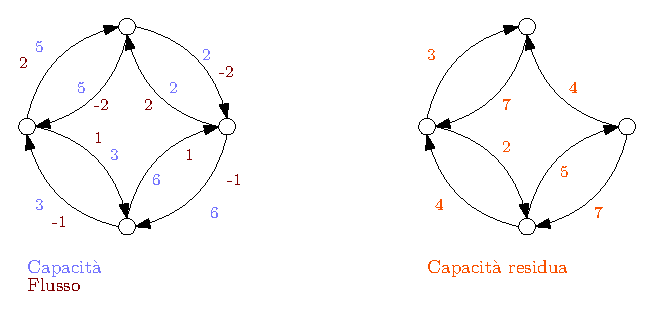
\includegraphics[width=0.7\textwidth ]{images/residual_graph.eps}
    \caption{Capacità residua del flusso (evidenziato in rosso)}
\end{figure}
Si assuma che esiste un cammino $P$ in $G'$ da $s$ a $t$, si consideri il residuo minimo valutato sugli archi contenuti nel cammino 
$$ \alpha=\min_{(u,v)\in E(P)}r(u,v)$$
Si definisce una funzione $f':E(G)\rightarrow\R$ come segue $$ f'(u,v)=\begin{cases}
    f(u,v)+\alpha  \ \text{ se } \ (u,v)\in E(P) \\
    f(u,v)-\alpha  \ \text{ se } \ (v,u) \in E(P)\\
    f(u,v)  \ \text{ altrimenti } 
\end{cases}$$
\begin{proposizione}
$f'$ è un flusso per $G$.
\end{proposizione}
\textit{Dimostrazione} : Sia $(u,v)$ un arco in $G$, se $(u,v)\notin E(P)$, allora $f'(u,v)=f(u,v)$ e conseguentemente $f'(v,u)=f'(v,u)$, quindi la proprietà di skew simmetria è preservata. Differentemente, se $(u,v)\in E(P)$ si avrebbe che $f'(u,v)=f(u,v)+\alpha$ e $f'(v,u)=f(v,u)-\alpha=-f(u,v)-\alpha=-(f(u,v)+\alpha)$, quindi il nuovo flusso rispetta la proprietà di skew-simmetria. 

Per ogni arco $(u,v)\in E(P)$ si ha che $f'(u,v)=f(u,v)+\alpha$, $\alpha$ è (per definizione) minore o uguale a $r(u,v)$ quindi 
$$ f'(u,v)\le f(u,v)+r(u,v)$$
Ma essendo che $f(u,v)+r(u,v)=c(u,v)$, $f'$ rispetta la capacità.

Se $x\notin V(P)$ si avrebbe che $f'(x,u)=f(x,u)$ per ogni $u$ adiacente ad $x$, allora $$ \sum_{(x,u)\in E(G)}f(x,u)=0$$
Assumendo che $x\in V(P)$,  vi è un arco uscente da $x$ il cui flusso è aumentato di $\alpha$, vi è quindi (per definizione di $f'$) un'arco entrante in $x$ il cui flusso è diminuito di $\alpha$, quindi è ancora vero che
$$ \sum_{\begin{matrix}(u,x)\in E(G)\\f'(u,x)>0\end{matrix}}f'(u,x)=-\Bigg(
\sum_{\begin{matrix}(x,u)\in E(G)\\f'(x,u)<0\end{matrix}}f'(x,u)\Bigg)$$
la proprietà di conservazione del flusso è rispettata.\hfill$\blacksquare$\bigskip 

Il valore del nuovo flusso è uguale al valore del flusso di partenza aumentato di $\alpha$ 
$$ \text{val}(f')=\text{val}(f)+\alpha$$
Dato che un singolo arco $(s,u)$ per qualche $u$ è necessariamente presente nel cammino $P$ da $s$ a $t$, ed il valore di $f'$ su $(s,u)$ è stato aumentato di $\alpha$.
\end{document}